\documentclass[11pt]{article}

    \usepackage[breakable]{tcolorbox}
    \usepackage{parskip} % Stop auto-indenting (to mimic markdown behaviour)
    \usepackage{fontspec, xunicode, xltxtra}
	\setmainfont{Microsoft YaHei}
	\usepackage{ctex}

    % Basic figure setup, for now with no caption control since it's done
    % automatically by Pandoc (which extracts ![](path) syntax from Markdown).
    \usepackage{graphicx}
    % Maintain compatibility with old templates. Remove in nbconvert 6.0
    \let\Oldincludegraphics\includegraphics
    % Ensure that by default, figures have no caption (until we provide a
    % proper Figure object with a Caption API and a way to capture that
    % in the conversion process - todo).
    \usepackage{caption}
    \DeclareCaptionFormat{nocaption}{}
    \captionsetup{format=nocaption,aboveskip=0pt,belowskip=0pt}

    \usepackage{float}
    \floatplacement{figure}{H} % forces figures to be placed at the correct location
    \usepackage{xcolor} % Allow colors to be defined
    \usepackage{enumerate} % Needed for markdown enumerations to work
    \usepackage{geometry} % Used to adjust the document margins
    \usepackage{amsmath} % Equations
    \usepackage{amssymb} % Equations
    \usepackage{textcomp} % defines textquotesingle
    % Hack from http://tex.stackexchange.com/a/47451/13684:
    \AtBeginDocument{%
        \def\PYZsq{\textquotesingle}% Upright quotes in Pygmentized code
    }
    \usepackage{upquote} % Upright quotes for verbatim code
    \usepackage{eurosym} % defines \euro

    \usepackage{iftex}
    \ifPDFTeX
        \usepackage[T1]{fontenc}
        \IfFileExists{alphabeta.sty}{
              \usepackage{alphabeta}
          }{
              \usepackage[mathletters]{ucs}
              \usepackage[utf8x]{inputenc}
          }
    \else
        \usepackage{fontspec}
        \usepackage{unicode-math}
    \fi

    \usepackage{fancyvrb} % verbatim replacement that allows latex
    \usepackage{grffile} % extends the file name processing of package graphics
                         % to support a larger range
    \makeatletter % fix for old versions of grffile with XeLaTeX
    \@ifpackagelater{grffile}{2019/11/01}
    {
      % Do nothing on new versions
    }
    {
      \def\Gread@@xetex#1{%
        \IfFileExists{"\Gin@base".bb}%
        {\Gread@eps{\Gin@base.bb}}%
        {\Gread@@xetex@aux#1}%
      }
    }
    \makeatother
    \usepackage[Export]{adjustbox} % Used to constrain images to a maximum size
    \adjustboxset{max size={0.9\linewidth}{0.9\paperheight}}

    % The hyperref package gives us a pdf with properly built
    % internal navigation ('pdf bookmarks' for the table of contents,
    % internal cross-reference links, web links for URLs, etc.)
    \usepackage{hyperref}
    % The default LaTeX title has an obnoxious amount of whitespace. By default,
    % titling removes some of it. It also provides customization options.
    \usepackage{titling}
    \usepackage{longtable} % longtable support required by pandoc >1.10
    \usepackage{booktabs}  % table support for pandoc > 1.12.2
    \usepackage{array}     % table support for pandoc >= 2.11.3
    \usepackage{calc}      % table minipage width calculation for pandoc >= 2.11.1
    \usepackage[inline]{enumitem} % IRkernel/repr support (it uses the enumerate* environment)
    \usepackage[normalem]{ulem} % ulem is needed to support strikethroughs (\sout)
                                % normalem makes italics be italics, not underlines
    \usepackage{mathrsfs}
    

    
    % Colors for the hyperref package
    \definecolor{urlcolor}{rgb}{0,.145,.698}
    \definecolor{linkcolor}{rgb}{.71,0.21,0.01}
    \definecolor{citecolor}{rgb}{.12,.54,.11}

    % ANSI colors
    \definecolor{ansi-black}{HTML}{3E424D}
    \definecolor{ansi-black-intense}{HTML}{282C36}
    \definecolor{ansi-red}{HTML}{E75C58}
    \definecolor{ansi-red-intense}{HTML}{B22B31}
    \definecolor{ansi-green}{HTML}{00A250}
    \definecolor{ansi-green-intense}{HTML}{007427}
    \definecolor{ansi-yellow}{HTML}{DDB62B}
    \definecolor{ansi-yellow-intense}{HTML}{B27D12}
    \definecolor{ansi-blue}{HTML}{208FFB}
    \definecolor{ansi-blue-intense}{HTML}{0065CA}
    \definecolor{ansi-magenta}{HTML}{D160C4}
    \definecolor{ansi-magenta-intense}{HTML}{A03196}
    \definecolor{ansi-cyan}{HTML}{60C6C8}
    \definecolor{ansi-cyan-intense}{HTML}{258F8F}
    \definecolor{ansi-white}{HTML}{C5C1B4}
    \definecolor{ansi-white-intense}{HTML}{A1A6B2}
    \definecolor{ansi-default-inverse-fg}{HTML}{FFFFFF}
    \definecolor{ansi-default-inverse-bg}{HTML}{000000}

    % common color for the border for error outputs.
    \definecolor{outerrorbackground}{HTML}{FFDFDF}

    % commands and environments needed by pandoc snippets
    % extracted from the output of `pandoc -s`
    \providecommand{\tightlist}{%
      \setlength{\itemsep}{0pt}\setlength{\parskip}{0pt}}
    \DefineVerbatimEnvironment{Highlighting}{Verbatim}{commandchars=\\\{\}}
    % Add ',fontsize=\small' for more characters per line
    \newenvironment{Shaded}{}{}
    \newcommand{\KeywordTok}[1]{\textcolor[rgb]{0.00,0.44,0.13}{\textbf{{#1}}}}
    \newcommand{\DataTypeTok}[1]{\textcolor[rgb]{0.56,0.13,0.00}{{#1}}}
    \newcommand{\DecValTok}[1]{\textcolor[rgb]{0.25,0.63,0.44}{{#1}}}
    \newcommand{\BaseNTok}[1]{\textcolor[rgb]{0.25,0.63,0.44}{{#1}}}
    \newcommand{\FloatTok}[1]{\textcolor[rgb]{0.25,0.63,0.44}{{#1}}}
    \newcommand{\CharTok}[1]{\textcolor[rgb]{0.25,0.44,0.63}{{#1}}}
    \newcommand{\StringTok}[1]{\textcolor[rgb]{0.25,0.44,0.63}{{#1}}}
    \newcommand{\CommentTok}[1]{\textcolor[rgb]{0.38,0.63,0.69}{\textit{{#1}}}}
    \newcommand{\OtherTok}[1]{\textcolor[rgb]{0.00,0.44,0.13}{{#1}}}
    \newcommand{\AlertTok}[1]{\textcolor[rgb]{1.00,0.00,0.00}{\textbf{{#1}}}}
    \newcommand{\FunctionTok}[1]{\textcolor[rgb]{0.02,0.16,0.49}{{#1}}}
    \newcommand{\RegionMarkerTok}[1]{{#1}}
    \newcommand{\ErrorTok}[1]{\textcolor[rgb]{1.00,0.00,0.00}{\textbf{{#1}}}}
    \newcommand{\NormalTok}[1]{{#1}}

    % Additional commands for more recent versions of Pandoc
    \newcommand{\ConstantTok}[1]{\textcolor[rgb]{0.53,0.00,0.00}{{#1}}}
    \newcommand{\SpecialCharTok}[1]{\textcolor[rgb]{0.25,0.44,0.63}{{#1}}}
    \newcommand{\VerbatimStringTok}[1]{\textcolor[rgb]{0.25,0.44,0.63}{{#1}}}
    \newcommand{\SpecialStringTok}[1]{\textcolor[rgb]{0.73,0.40,0.53}{{#1}}}
    \newcommand{\ImportTok}[1]{{#1}}
    \newcommand{\DocumentationTok}[1]{\textcolor[rgb]{0.73,0.13,0.13}{\textit{{#1}}}}
    \newcommand{\AnnotationTok}[1]{\textcolor[rgb]{0.38,0.63,0.69}{\textbf{\textit{{#1}}}}}
    \newcommand{\CommentVarTok}[1]{\textcolor[rgb]{0.38,0.63,0.69}{\textbf{\textit{{#1}}}}}
    \newcommand{\VariableTok}[1]{\textcolor[rgb]{0.10,0.09,0.49}{{#1}}}
    \newcommand{\ControlFlowTok}[1]{\textcolor[rgb]{0.00,0.44,0.13}{\textbf{{#1}}}}
    \newcommand{\OperatorTok}[1]{\textcolor[rgb]{0.40,0.40,0.40}{{#1}}}
    \newcommand{\BuiltInTok}[1]{{#1}}
    \newcommand{\ExtensionTok}[1]{{#1}}
    \newcommand{\PreprocessorTok}[1]{\textcolor[rgb]{0.74,0.48,0.00}{{#1}}}
    \newcommand{\AttributeTok}[1]{\textcolor[rgb]{0.49,0.56,0.16}{{#1}}}
    \newcommand{\InformationTok}[1]{\textcolor[rgb]{0.38,0.63,0.69}{\textbf{\textit{{#1}}}}}
    \newcommand{\WarningTok}[1]{\textcolor[rgb]{0.38,0.63,0.69}{\textbf{\textit{{#1}}}}}


    % Define a nice break command that doesn't care if a line doesn't already
    % exist.
    \def\br{\hspace*{\fill} \\* }
    % Math Jax compatibility definitions
    \def\gt{>}
    \def\lt{<}
    \let\Oldtex\TeX
    \let\Oldlatex\LaTeX
    \renewcommand{\TeX}{\textrm{\Oldtex}}
    \renewcommand{\LaTeX}{\textrm{\Oldlatex}}
    % Document parameters
    % Document title
    \title{lab\_1}
    
    
    
    
    
% Pygments definitions
\makeatletter
\def\PY@reset{\let\PY@it=\relax \let\PY@bf=\relax%
    \let\PY@ul=\relax \let\PY@tc=\relax%
    \let\PY@bc=\relax \let\PY@ff=\relax}
\def\PY@tok#1{\csname PY@tok@#1\endcsname}
\def\PY@toks#1+{\ifx\relax#1\empty\else%
    \PY@tok{#1}\expandafter\PY@toks\fi}
\def\PY@do#1{\PY@bc{\PY@tc{\PY@ul{%
    \PY@it{\PY@bf{\PY@ff{#1}}}}}}}
\def\PY#1#2{\PY@reset\PY@toks#1+\relax+\PY@do{#2}}

\@namedef{PY@tok@w}{\def\PY@tc##1{\textcolor[rgb]{0.73,0.73,0.73}{##1}}}
\@namedef{PY@tok@c}{\let\PY@it=\textit\def\PY@tc##1{\textcolor[rgb]{0.24,0.48,0.48}{##1}}}
\@namedef{PY@tok@cp}{\def\PY@tc##1{\textcolor[rgb]{0.61,0.40,0.00}{##1}}}
\@namedef{PY@tok@k}{\let\PY@bf=\textbf\def\PY@tc##1{\textcolor[rgb]{0.00,0.50,0.00}{##1}}}
\@namedef{PY@tok@kp}{\def\PY@tc##1{\textcolor[rgb]{0.00,0.50,0.00}{##1}}}
\@namedef{PY@tok@kt}{\def\PY@tc##1{\textcolor[rgb]{0.69,0.00,0.25}{##1}}}
\@namedef{PY@tok@o}{\def\PY@tc##1{\textcolor[rgb]{0.40,0.40,0.40}{##1}}}
\@namedef{PY@tok@ow}{\let\PY@bf=\textbf\def\PY@tc##1{\textcolor[rgb]{0.67,0.13,1.00}{##1}}}
\@namedef{PY@tok@nb}{\def\PY@tc##1{\textcolor[rgb]{0.00,0.50,0.00}{##1}}}
\@namedef{PY@tok@nf}{\def\PY@tc##1{\textcolor[rgb]{0.00,0.00,1.00}{##1}}}
\@namedef{PY@tok@nc}{\let\PY@bf=\textbf\def\PY@tc##1{\textcolor[rgb]{0.00,0.00,1.00}{##1}}}
\@namedef{PY@tok@nn}{\let\PY@bf=\textbf\def\PY@tc##1{\textcolor[rgb]{0.00,0.00,1.00}{##1}}}
\@namedef{PY@tok@ne}{\let\PY@bf=\textbf\def\PY@tc##1{\textcolor[rgb]{0.80,0.25,0.22}{##1}}}
\@namedef{PY@tok@nv}{\def\PY@tc##1{\textcolor[rgb]{0.10,0.09,0.49}{##1}}}
\@namedef{PY@tok@no}{\def\PY@tc##1{\textcolor[rgb]{0.53,0.00,0.00}{##1}}}
\@namedef{PY@tok@nl}{\def\PY@tc##1{\textcolor[rgb]{0.46,0.46,0.00}{##1}}}
\@namedef{PY@tok@ni}{\let\PY@bf=\textbf\def\PY@tc##1{\textcolor[rgb]{0.44,0.44,0.44}{##1}}}
\@namedef{PY@tok@na}{\def\PY@tc##1{\textcolor[rgb]{0.41,0.47,0.13}{##1}}}
\@namedef{PY@tok@nt}{\let\PY@bf=\textbf\def\PY@tc##1{\textcolor[rgb]{0.00,0.50,0.00}{##1}}}
\@namedef{PY@tok@nd}{\def\PY@tc##1{\textcolor[rgb]{0.67,0.13,1.00}{##1}}}
\@namedef{PY@tok@s}{\def\PY@tc##1{\textcolor[rgb]{0.73,0.13,0.13}{##1}}}
\@namedef{PY@tok@sd}{\let\PY@it=\textit\def\PY@tc##1{\textcolor[rgb]{0.73,0.13,0.13}{##1}}}
\@namedef{PY@tok@si}{\let\PY@bf=\textbf\def\PY@tc##1{\textcolor[rgb]{0.64,0.35,0.47}{##1}}}
\@namedef{PY@tok@se}{\let\PY@bf=\textbf\def\PY@tc##1{\textcolor[rgb]{0.67,0.36,0.12}{##1}}}
\@namedef{PY@tok@sr}{\def\PY@tc##1{\textcolor[rgb]{0.64,0.35,0.47}{##1}}}
\@namedef{PY@tok@ss}{\def\PY@tc##1{\textcolor[rgb]{0.10,0.09,0.49}{##1}}}
\@namedef{PY@tok@sx}{\def\PY@tc##1{\textcolor[rgb]{0.00,0.50,0.00}{##1}}}
\@namedef{PY@tok@m}{\def\PY@tc##1{\textcolor[rgb]{0.40,0.40,0.40}{##1}}}
\@namedef{PY@tok@gh}{\let\PY@bf=\textbf\def\PY@tc##1{\textcolor[rgb]{0.00,0.00,0.50}{##1}}}
\@namedef{PY@tok@gu}{\let\PY@bf=\textbf\def\PY@tc##1{\textcolor[rgb]{0.50,0.00,0.50}{##1}}}
\@namedef{PY@tok@gd}{\def\PY@tc##1{\textcolor[rgb]{0.63,0.00,0.00}{##1}}}
\@namedef{PY@tok@gi}{\def\PY@tc##1{\textcolor[rgb]{0.00,0.52,0.00}{##1}}}
\@namedef{PY@tok@gr}{\def\PY@tc##1{\textcolor[rgb]{0.89,0.00,0.00}{##1}}}
\@namedef{PY@tok@ge}{\let\PY@it=\textit}
\@namedef{PY@tok@gs}{\let\PY@bf=\textbf}
\@namedef{PY@tok@gp}{\let\PY@bf=\textbf\def\PY@tc##1{\textcolor[rgb]{0.00,0.00,0.50}{##1}}}
\@namedef{PY@tok@go}{\def\PY@tc##1{\textcolor[rgb]{0.44,0.44,0.44}{##1}}}
\@namedef{PY@tok@gt}{\def\PY@tc##1{\textcolor[rgb]{0.00,0.27,0.87}{##1}}}
\@namedef{PY@tok@err}{\def\PY@bc##1{{\setlength{\fboxsep}{\string -\fboxrule}\fcolorbox[rgb]{1.00,0.00,0.00}{1,1,1}{\strut ##1}}}}
\@namedef{PY@tok@kc}{\let\PY@bf=\textbf\def\PY@tc##1{\textcolor[rgb]{0.00,0.50,0.00}{##1}}}
\@namedef{PY@tok@kd}{\let\PY@bf=\textbf\def\PY@tc##1{\textcolor[rgb]{0.00,0.50,0.00}{##1}}}
\@namedef{PY@tok@kn}{\let\PY@bf=\textbf\def\PY@tc##1{\textcolor[rgb]{0.00,0.50,0.00}{##1}}}
\@namedef{PY@tok@kr}{\let\PY@bf=\textbf\def\PY@tc##1{\textcolor[rgb]{0.00,0.50,0.00}{##1}}}
\@namedef{PY@tok@bp}{\def\PY@tc##1{\textcolor[rgb]{0.00,0.50,0.00}{##1}}}
\@namedef{PY@tok@fm}{\def\PY@tc##1{\textcolor[rgb]{0.00,0.00,1.00}{##1}}}
\@namedef{PY@tok@vc}{\def\PY@tc##1{\textcolor[rgb]{0.10,0.09,0.49}{##1}}}
\@namedef{PY@tok@vg}{\def\PY@tc##1{\textcolor[rgb]{0.10,0.09,0.49}{##1}}}
\@namedef{PY@tok@vi}{\def\PY@tc##1{\textcolor[rgb]{0.10,0.09,0.49}{##1}}}
\@namedef{PY@tok@vm}{\def\PY@tc##1{\textcolor[rgb]{0.10,0.09,0.49}{##1}}}
\@namedef{PY@tok@sa}{\def\PY@tc##1{\textcolor[rgb]{0.73,0.13,0.13}{##1}}}
\@namedef{PY@tok@sb}{\def\PY@tc##1{\textcolor[rgb]{0.73,0.13,0.13}{##1}}}
\@namedef{PY@tok@sc}{\def\PY@tc##1{\textcolor[rgb]{0.73,0.13,0.13}{##1}}}
\@namedef{PY@tok@dl}{\def\PY@tc##1{\textcolor[rgb]{0.73,0.13,0.13}{##1}}}
\@namedef{PY@tok@s2}{\def\PY@tc##1{\textcolor[rgb]{0.73,0.13,0.13}{##1}}}
\@namedef{PY@tok@sh}{\def\PY@tc##1{\textcolor[rgb]{0.73,0.13,0.13}{##1}}}
\@namedef{PY@tok@s1}{\def\PY@tc##1{\textcolor[rgb]{0.73,0.13,0.13}{##1}}}
\@namedef{PY@tok@mb}{\def\PY@tc##1{\textcolor[rgb]{0.40,0.40,0.40}{##1}}}
\@namedef{PY@tok@mf}{\def\PY@tc##1{\textcolor[rgb]{0.40,0.40,0.40}{##1}}}
\@namedef{PY@tok@mh}{\def\PY@tc##1{\textcolor[rgb]{0.40,0.40,0.40}{##1}}}
\@namedef{PY@tok@mi}{\def\PY@tc##1{\textcolor[rgb]{0.40,0.40,0.40}{##1}}}
\@namedef{PY@tok@il}{\def\PY@tc##1{\textcolor[rgb]{0.40,0.40,0.40}{##1}}}
\@namedef{PY@tok@mo}{\def\PY@tc##1{\textcolor[rgb]{0.40,0.40,0.40}{##1}}}
\@namedef{PY@tok@ch}{\let\PY@it=\textit\def\PY@tc##1{\textcolor[rgb]{0.24,0.48,0.48}{##1}}}
\@namedef{PY@tok@cm}{\let\PY@it=\textit\def\PY@tc##1{\textcolor[rgb]{0.24,0.48,0.48}{##1}}}
\@namedef{PY@tok@cpf}{\let\PY@it=\textit\def\PY@tc##1{\textcolor[rgb]{0.24,0.48,0.48}{##1}}}
\@namedef{PY@tok@c1}{\let\PY@it=\textit\def\PY@tc##1{\textcolor[rgb]{0.24,0.48,0.48}{##1}}}
\@namedef{PY@tok@cs}{\let\PY@it=\textit\def\PY@tc##1{\textcolor[rgb]{0.24,0.48,0.48}{##1}}}

\def\PYZbs{\char`\\}
\def\PYZus{\char`\_}
\def\PYZob{\char`\{}
\def\PYZcb{\char`\}}
\def\PYZca{\char`\^}
\def\PYZam{\char`\&}
\def\PYZlt{\char`\<}
\def\PYZgt{\char`\>}
\def\PYZsh{\char`\#}
\def\PYZpc{\char`\%}
\def\PYZdl{\char`\$}
\def\PYZhy{\char`\-}
\def\PYZsq{\char`\'}
\def\PYZdq{\char`\"}
\def\PYZti{\char`\~}
% for compatibility with earlier versions
\def\PYZat{@}
\def\PYZlb{[}
\def\PYZrb{]}
\makeatother


    % For linebreaks inside Verbatim environment from package fancyvrb.
    \makeatletter
        \newbox\Wrappedcontinuationbox
        \newbox\Wrappedvisiblespacebox
        \newcommand*\Wrappedvisiblespace {\textcolor{red}{\textvisiblespace}}
        \newcommand*\Wrappedcontinuationsymbol {\textcolor{red}{\llap{\tiny$\m@th\hookrightarrow$}}}
        \newcommand*\Wrappedcontinuationindent {3ex }
        \newcommand*\Wrappedafterbreak {\kern\Wrappedcontinuationindent\copy\Wrappedcontinuationbox}
        % Take advantage of the already applied Pygments mark-up to insert
        % potential linebreaks for TeX processing.
        %        {, <, #, %, $, ' and ": go to next line.
        %        _, }, ^, &, >, - and ~: stay at end of broken line.
        % Use of \textquotesingle for straight quote.
        \newcommand*\Wrappedbreaksatspecials {%
            \def\PYGZus{\discretionary{\char`\_}{\Wrappedafterbreak}{\char`\_}}%
            \def\PYGZob{\discretionary{}{\Wrappedafterbreak\char`\{}{\char`\{}}%
            \def\PYGZcb{\discretionary{\char`\}}{\Wrappedafterbreak}{\char`\}}}%
            \def\PYGZca{\discretionary{\char`\^}{\Wrappedafterbreak}{\char`\^}}%
            \def\PYGZam{\discretionary{\char`\&}{\Wrappedafterbreak}{\char`\&}}%
            \def\PYGZlt{\discretionary{}{\Wrappedafterbreak\char`\<}{\char`\<}}%
            \def\PYGZgt{\discretionary{\char`\>}{\Wrappedafterbreak}{\char`\>}}%
            \def\PYGZsh{\discretionary{}{\Wrappedafterbreak\char`\#}{\char`\#}}%
            \def\PYGZpc{\discretionary{}{\Wrappedafterbreak\char`\%}{\char`\%}}%
            \def\PYGZdl{\discretionary{}{\Wrappedafterbreak\char`\$}{\char`\$}}%
            \def\PYGZhy{\discretionary{\char`\-}{\Wrappedafterbreak}{\char`\-}}%
            \def\PYGZsq{\discretionary{}{\Wrappedafterbreak\textquotesingle}{\textquotesingle}}%
            \def\PYGZdq{\discretionary{}{\Wrappedafterbreak\char`\"}{\char`\"}}%
            \def\PYGZti{\discretionary{\char`\~}{\Wrappedafterbreak}{\char`\~}}%
        }
        % Some characters . , ; ? ! / are not pygmentized.
        % This macro makes them "active" and they will insert potential linebreaks
        \newcommand*\Wrappedbreaksatpunct {%
            \lccode`\~`\.\lowercase{\def~}{\discretionary{\hbox{\char`\.}}{\Wrappedafterbreak}{\hbox{\char`\.}}}%
            \lccode`\~`\,\lowercase{\def~}{\discretionary{\hbox{\char`\,}}{\Wrappedafterbreak}{\hbox{\char`\,}}}%
            \lccode`\~`\;\lowercase{\def~}{\discretionary{\hbox{\char`\;}}{\Wrappedafterbreak}{\hbox{\char`\;}}}%
            \lccode`\~`\:\lowercase{\def~}{\discretionary{\hbox{\char`\:}}{\Wrappedafterbreak}{\hbox{\char`\:}}}%
            \lccode`\~`\?\lowercase{\def~}{\discretionary{\hbox{\char`\?}}{\Wrappedafterbreak}{\hbox{\char`\?}}}%
            \lccode`\~`\!\lowercase{\def~}{\discretionary{\hbox{\char`\!}}{\Wrappedafterbreak}{\hbox{\char`\!}}}%
            \lccode`\~`\/\lowercase{\def~}{\discretionary{\hbox{\char`\/}}{\Wrappedafterbreak}{\hbox{\char`\/}}}%
            \catcode`\.\active
            \catcode`\,\active
            \catcode`\;\active
            \catcode`\:\active
            \catcode`\?\active
            \catcode`\!\active
            \catcode`\/\active
            \lccode`\~`\~
        }
    \makeatother

    \let\OriginalVerbatim=\Verbatim
    \makeatletter
    \renewcommand{\Verbatim}[1][1]{%
        %\parskip\z@skip
        \sbox\Wrappedcontinuationbox {\Wrappedcontinuationsymbol}%
        \sbox\Wrappedvisiblespacebox {\FV@SetupFont\Wrappedvisiblespace}%
        \def\FancyVerbFormatLine ##1{\hsize\linewidth
            \vtop{\raggedright\hyphenpenalty\z@\exhyphenpenalty\z@
                \doublehyphendemerits\z@\finalhyphendemerits\z@
                \strut ##1\strut}%
        }%
        % If the linebreak is at a space, the latter will be displayed as visible
        % space at end of first line, and a continuation symbol starts next line.
        % Stretch/shrink are however usually zero for typewriter font.
        \def\FV@Space {%
            \nobreak\hskip\z@ plus\fontdimen3\font minus\fontdimen4\font
            \discretionary{\copy\Wrappedvisiblespacebox}{\Wrappedafterbreak}
            {\kern\fontdimen2\font}%
        }%

        % Allow breaks at special characters using \PYG... macros.
        \Wrappedbreaksatspecials
        % Breaks at punctuation characters . , ; ? ! and / need catcode=\active
        \OriginalVerbatim[#1,codes*=\Wrappedbreaksatpunct]%
    }
    \makeatother

    % Exact colors from NB
    \definecolor{incolor}{HTML}{303F9F}
    \definecolor{outcolor}{HTML}{D84315}
    \definecolor{cellborder}{HTML}{CFCFCF}
    \definecolor{cellbackground}{HTML}{F7F7F7}

    % prompt
    \makeatletter
    \newcommand{\boxspacing}{\kern\kvtcb@left@rule\kern\kvtcb@boxsep}
    \makeatother
    \newcommand{\prompt}[4]{
        {\ttfamily\llap{{\color{#2}[#3]:\hspace{3pt}#4}}\vspace{-\baselineskip}}
    }
    

    
    % Prevent overflowing lines due to hard-to-break entities
    \sloppy
    % Setup hyperref package
    \hypersetup{
      breaklinks=true,  % so long urls are correctly broken across lines
      colorlinks=true,
      urlcolor=urlcolor,
      linkcolor=linkcolor,
      citecolor=citecolor,
      }
    % Slightly bigger margins than the latex defaults
    
    \geometry{verbose,tmargin=1in,bmargin=1in,lmargin=1in,rmargin=1in}
    
    

\begin{document}
    
    \maketitle
    
    

    
    \hypertarget{ux5b9eux9a8cux4e00-lab-1-ux63d2ux5165ux6392ux5e8fux4e0eux5f52ux5e76ux6392ux5e8fux7684ux5b9eux9a8cux6027ux80fdux6bd4ux8f83}{%
\section{实验一 · Lab 1 ·
插入排序与归并排序的实验性能比较}\label{ux5b9eux9a8cux4e00-lab-1-ux63d2ux5165ux6392ux5e8fux4e0eux5f52ux5e76ux6392ux5e8fux7684ux5b9eux9a8cux6027ux80fdux6bd4ux8f83}}

\hypertarget{ux9700ux6c42ux5206ux6790}{%
\subsection{需求分析}\label{ux9700ux6c42ux5206ux6790}}

\begin{itemize}
\tightlist
\item
  输入:规模为n的测试集(列表,n分别取10k,20k,30k,40k,50k)
\item
  输出:排序过后的顺序集,以及不同规模下、不同排序方法的消耗时间
\item
  程序功能:

  \begin{itemize}
  \tightlist
  \item
    针对每一个输入规模n,随机产生10组测试样本,统计两种不同排序算法在10个样本上的平均运行时间;画出这两种不同排序算法在10个随机样本的平均运行时间与输入规模n的关系
  \item
    画出理论效率分析的曲线和实测的效率曲线
  \end{itemize}
\item
  测试集:由于取特定值的操作时间复杂度在同一数据结构中保持一致,在对不同数据结构进行排序操作通常不考虑取值时间。则为方便测试,本实验测试集均为整数(int)
\end{itemize}

\hypertarget{ux8be6ux7ec6ux8bbeux8ba1ux4e0eux5b9eux9a8c}{%
\subsection{详细设计与实验}\label{ux8be6ux7ec6ux8bbeux8ba1ux4e0eux5b9eux9a8c}}

\hypertarget{ux63d2ux5165ux6392ux5e8fux4e0eux5f52ux5e76ux6392ux5e8f-ux51fdux6570ux5b9eux73b0python}{%
\subsubsection{插入排序与归并排序
函数实现(python)}\label{ux63d2ux5165ux6392ux5e8fux4e0eux5f52ux5e76ux6392ux5e8f-ux51fdux6570ux5b9eux73b0python}}

    \begin{tcolorbox}[breakable, size=fbox, boxrule=1pt, pad at break*=1mm,colback=cellbackground, colframe=cellborder]
\prompt{In}{incolor}{55}{\boxspacing}
\begin{Verbatim}[commandchars=\\\{\}]
\PY{c+c1}{\PYZsh{} @param    arr     需要排序的序列数组}
\PY{c+c1}{\PYZsh{} @param    start   排序序列的初始index,一般为0}
\PY{c+c1}{\PYZsh{} @param    end     排序序列的结尾index,注意不是数组长度}
\PY{k}{def} \PY{n+nf}{sort\PYZus{}insertion}\PY{p}{(}\PY{n}{arr}\PY{p}{,}\PY{n}{start}\PY{p}{,}\PY{n}{end}\PY{p}{)}\PY{p}{:} \PY{c+c1}{\PYZsh{} 插入排序算法}
    \PY{k}{for} \PY{n}{j} \PY{o+ow}{in} \PY{n+nb}{range}\PY{p}{(}\PY{n}{start}\PY{o}{+}\PY{l+m+mi}{1}\PY{p}{,}\PY{n}{end}\PY{o}{+}\PY{l+m+mi}{1}\PY{p}{)}\PY{p}{:}
        \PY{n}{key} \PY{o}{=} \PY{n}{arr}\PY{p}{[}\PY{n}{j}\PY{p}{]}
        \PY{n}{i} \PY{o}{=} \PY{n}{j} \PY{o}{\PYZhy{}} \PY{l+m+mi}{1}
        \PY{k}{while} \PY{p}{(}\PY{n}{i} \PY{o}{\PYZgt{}}\PY{o}{=} \PY{l+m+mi}{0}\PY{p}{)} \PY{o+ow}{and} \PY{p}{(}\PY{n}{arr}\PY{p}{[}\PY{n}{i}\PY{p}{]} \PY{o}{\PYZgt{}} \PY{n}{key}\PY{p}{)}\PY{p}{:}
            \PY{n}{arr}\PY{p}{[}\PY{n}{i}\PY{o}{+}\PY{l+m+mi}{1}\PY{p}{]} \PY{o}{=} \PY{n}{arr}\PY{p}{[}\PY{n}{i}\PY{p}{]}
            \PY{n}{i} \PY{o}{\PYZhy{}}\PY{o}{=} \PY{l+m+mi}{1}
        \PY{n}{arr}\PY{p}{[}\PY{n}{i}\PY{o}{+}\PY{l+m+mi}{1}\PY{p}{]} \PY{o}{=} \PY{n}{key}


\PY{c+c1}{\PYZsh{} @param    arr     需要合并的序列数组}
\PY{c+c1}{\PYZsh{} @param    p       合并序列的初始index,一般为0}
\PY{c+c1}{\PYZsh{} @param    q       合并序列的中间index}
\PY{c+c1}{\PYZsh{} @param    r       合并序列的末尾index}
\PY{k}{def} \PY{n+nf}{merge}\PY{p}{(}\PY{n}{arr}\PY{p}{,}\PY{n}{p}\PY{p}{,}\PY{n}{q}\PY{p}{,}\PY{n}{r}\PY{p}{)}\PY{p}{:}   \PY{c+c1}{\PYZsh{} 归并函数(加入哨兵,简化代码)}
    \PY{n}{leftArr} \PY{o}{=} \PY{n}{arr}\PY{p}{[}\PY{n}{p}\PY{p}{:}\PY{n}{q}\PY{o}{+}\PY{l+m+mi}{1}\PY{p}{]}
    \PY{n}{rightArr} \PY{o}{=} \PY{n}{arr}\PY{p}{[}\PY{n}{q}\PY{o}{+}\PY{l+m+mi}{1}\PY{p}{:}\PY{n}{r}\PY{o}{+}\PY{l+m+mi}{1}\PY{p}{]}

    \PY{n}{leftArr}\PY{o}{.}\PY{n}{append}\PY{p}{(}\PY{n+nb}{float}\PY{p}{(}\PY{l+s+s1}{\PYZsq{}}\PY{l+s+s1}{inf}\PY{l+s+s1}{\PYZsq{}}\PY{p}{)}\PY{p}{)}
    \PY{n}{rightArr}\PY{o}{.}\PY{n}{append}\PY{p}{(}\PY{n+nb}{float}\PY{p}{(}\PY{l+s+s1}{\PYZsq{}}\PY{l+s+s1}{inf}\PY{l+s+s1}{\PYZsq{}}\PY{p}{)}\PY{p}{)}

    \PY{n}{i} \PY{o}{=} \PY{l+m+mi}{0}
    \PY{n}{j} \PY{o}{=} \PY{l+m+mi}{0}
    \PY{k}{for} \PY{n}{k} \PY{o+ow}{in} \PY{n+nb}{range}\PY{p}{(}\PY{n}{p}\PY{p}{,}\PY{n}{r}\PY{o}{+}\PY{l+m+mi}{1}\PY{p}{)}\PY{p}{:}
        \PY{k}{if} \PY{n}{leftArr}\PY{p}{[}\PY{n}{i}\PY{p}{]} \PY{o}{\PYZlt{}}\PY{o}{=} \PY{n}{rightArr}\PY{p}{[}\PY{n}{j}\PY{p}{]}\PY{p}{:}
            \PY{n}{arr}\PY{p}{[}\PY{n}{k}\PY{p}{]} \PY{o}{=} \PY{n}{leftArr}\PY{p}{[}\PY{n}{i}\PY{p}{]}
            \PY{n}{i} \PY{o}{+}\PY{o}{=} \PY{l+m+mi}{1}
        \PY{k}{else}\PY{p}{:}
            \PY{n}{arr}\PY{p}{[}\PY{n}{k}\PY{p}{]} \PY{o}{=} \PY{n}{rightArr}\PY{p}{[}\PY{n}{j}\PY{p}{]}
            \PY{n}{j} \PY{o}{+}\PY{o}{=} \PY{l+m+mi}{1}


\PY{c+c1}{\PYZsh{} @param    arr     需要排序的序列数组}
\PY{c+c1}{\PYZsh{} @param    p       排序序列的初始index,一般为0}
\PY{c+c1}{\PYZsh{} @param    r       排序序列的结尾index,注意不是数组长度}
\PY{k}{def} \PY{n+nf}{sort\PYZus{}merge}\PY{p}{(}\PY{n}{arr}\PY{p}{,}\PY{n}{p}\PY{p}{,}\PY{n}{r}\PY{p}{)}\PY{p}{:}    \PY{c+c1}{\PYZsh{} 归并排序算法}
    \PY{k}{if} \PY{n}{p} \PY{o}{\PYZlt{}} \PY{n}{r}\PY{p}{:}
        \PY{n}{q} \PY{o}{=} \PY{p}{(}\PY{n}{p}\PY{o}{+}\PY{n}{r}\PY{p}{)}\PY{o}{/}\PY{o}{/}\PY{l+m+mi}{2}
        \PY{n}{sort\PYZus{}merge}\PY{p}{(}\PY{n}{arr}\PY{p}{,}\PY{n}{p}\PY{p}{,}\PY{n}{q}\PY{p}{)}
        \PY{n}{sort\PYZus{}merge}\PY{p}{(}\PY{n}{arr}\PY{p}{,}\PY{n}{q}\PY{o}{+}\PY{l+m+mi}{1}\PY{p}{,}\PY{n}{r}\PY{p}{)}
        \PY{n}{merge}\PY{p}{(}\PY{n}{arr}\PY{p}{,}\PY{n}{p}\PY{p}{,}\PY{n}{q}\PY{p}{,}\PY{n}{r}\PY{p}{)}
    \PY{k}{else}\PY{p}{:}
        \PY{k}{return}
\end{Verbatim}
\end{tcolorbox}

    \hypertarget{ux65f6ux95f4ux6548ux7387ux5206ux6790}{%
\subsubsection{时间效率分析}\label{ux65f6ux95f4ux6548ux7387ux5206ux6790}}

\hypertarget{ux63d2ux5165ux6392ux5e8f}{%
\paragraph{插入排序}\label{ux63d2ux5165ux6392ux5e8f}}

插入排序的基本操作是将一个元素插入到已经排好序的部分中,这一操作的时间复杂度取决于已排好序部分的长度,即插入位置的前面有多少个元素需要比较和移动。

假设要排序的序列长度为
n,那么在最坏情况下,每次插入操作都需要比较和移动整个已排序序列,因此第
i 个元素的插入操作时间复杂度为 i,总的时间复杂度为:

\[T(n) = 1 + 2 + 3 + ... + n-1
= \frac{n(n-1)}{2}
= O(n^{2})\]

\hypertarget{ux5f52ux5e76ux6392ux5e8f}{%
\paragraph{归并排序}\label{ux5f52ux5e76ux6392ux5e8f}}

归并分为两个步骤。首先是分治,将大序列分成数个不可分的元素。这个过程时间复杂度为
\[O(\log_2n)\],n为序列规模。
而第二个步骤为合并(merge),它是完整遍历整个序列,因此时间复杂度为
\[O(n)\]。

两者组合,时间复杂度相乘,则总的时间复杂度为: \[n \cdot \log_2n\]

    \hypertarget{ux751fux6210ux4e0dux540cux89c4ux6a21ux968fux673aux6574ux6570ux6d4bux8bd5ux96c6-ux51fdux6570ux5b9eux73b0}{%
\subsubsection{生成不同规模随机整数测试集
函数实现}\label{ux751fux6210ux4e0dux540cux89c4ux6a21ux968fux673aux6574ux6570ux6d4bux8bd5ux96c6-ux51fdux6570ux5b9eux73b0}}

    \begin{tcolorbox}[breakable, size=fbox, boxrule=1pt, pad at break*=1mm,colback=cellbackground, colframe=cellborder]
\prompt{In}{incolor}{56}{\boxspacing}
\begin{Verbatim}[commandchars=\\\{\}]
\PY{k+kn}{import} \PY{n+nn}{random}

\PY{n}{MAX\PYZus{}INT\PYZus{}NUMBER} \PY{o}{=} \PY{l+m+mi}{100000}     \PY{c+c1}{\PYZsh{} 随机数范围,暂定从0\PYZti{}10w}

\PY{c+c1}{\PYZsh{} @param n      测试集规模,生成n个随机数列表}

\PY{k}{def} \PY{n+nf}{generateTestSe\PYZus{}Int}\PY{p}{(}\PY{n}{n}\PY{p}{)}\PY{p}{:}
    \PY{n+nb}{list} \PY{o}{=} \PY{p}{[}\PY{p}{]}
    \PY{n}{i} \PY{o}{=} \PY{l+m+mi}{0}
    \PY{k}{while} \PY{n}{i} \PY{o}{\PYZlt{}} \PY{n}{n}\PY{p}{:}
        \PY{n+nb}{list}\PY{o}{.}\PY{n}{append}\PY{p}{(}\PY{n}{random}\PY{o}{.}\PY{n}{randint}\PY{p}{(}\PY{l+m+mi}{0}\PY{p}{,}\PY{n}{MAX\PYZus{}INT\PYZus{}NUMBER}\PY{p}{)}\PY{p}{)}
        \PY{n}{i} \PY{o}{+}\PY{o}{=} \PY{l+m+mi}{1}
    \PY{k}{return} \PY{n+nb}{list}
\end{Verbatim}
\end{tcolorbox}

    \hypertarget{ux8ba1ux7b97ux8fd0ux884cux65f6ux95f4ux5e76ux8fd4ux56de10ux6b21ux7ed3ux679cux5e73ux5747ux503c-ux51fdux6570ux5b9eux73b0}{%
\subsubsection{计算运行时间并返回10次结果平均值
函数实现}\label{ux8ba1ux7b97ux8fd0ux884cux65f6ux95f4ux5e76ux8fd4ux56de10ux6b21ux7ed3ux679cux5e73ux5747ux503c-ux51fdux6570ux5b9eux73b0}}

    \begin{tcolorbox}[breakable, size=fbox, boxrule=1pt, pad at break*=1mm,colback=cellbackground, colframe=cellborder]
\prompt{In}{incolor}{57}{\boxspacing}
\begin{Verbatim}[commandchars=\\\{\}]
\PY{k+kn}{import} \PY{n+nn}{time}

\PY{c+c1}{\PYZsh{} @param fun    具体排序函数指针}
\PY{c+c1}{\PYZsh{} @param n      测试集规模 如1e4\PYZhy{}\PYZgt{}10000}
\PY{c+c1}{\PYZsh{} @param k      计算次数,用于求平均值}

\PY{k}{def} \PY{n+nf}{returnCalculateRes\PYZus{}avg}\PY{p}{(}\PY{n}{fun}\PY{p}{,} \PY{n}{n}\PY{p}{,} \PY{n}{k}\PY{p}{)}\PY{p}{:}
    \PY{n+nb}{sum} \PY{o}{=} \PY{l+m+mi}{0}
    \PY{n}{i} \PY{o}{=} \PY{l+m+mi}{0}
    \PY{k}{while} \PY{n}{i} \PY{o}{\PYZlt{}} \PY{n}{k}\PY{p}{:}
        \PY{n+nb}{list} \PY{o}{=} \PY{n}{generateTestSe\PYZus{}Int}\PY{p}{(}\PY{n}{n}\PY{p}{)}
        \PY{n}{t1} \PY{o}{=} \PY{n}{time}\PY{o}{.}\PY{n}{perf\PYZus{}counter\PYZus{}ns}\PY{p}{(}\PY{p}{)}
        \PY{n}{fun}\PY{p}{(}\PY{n+nb}{list}\PY{p}{,}\PY{l+m+mi}{0}\PY{p}{,}\PY{n+nb}{len}\PY{p}{(}\PY{n+nb}{list}\PY{p}{)}\PY{o}{\PYZhy{}}\PY{l+m+mi}{1}\PY{p}{)}
        \PY{n}{t2} \PY{o}{=} \PY{n}{time}\PY{o}{.}\PY{n}{perf\PYZus{}counter\PYZus{}ns}\PY{p}{(}\PY{p}{)}
        \PY{n+nb}{sum} \PY{o}{+}\PY{o}{=} \PY{p}{(}\PY{n}{t2} \PY{o}{\PYZhy{}} \PY{n}{t1}\PY{p}{)}\PY{o}{/}\PY{l+m+mf}{1e6}
        \PY{n}{i} \PY{o}{+}\PY{o}{=} \PY{l+m+mi}{1}
    \PY{k}{return} \PY{n+nb}{sum}\PY{o}{/}\PY{n}{k}
\end{Verbatim}
\end{tcolorbox}

    \hypertarget{ux4e3bux4f53ux8fd0ux884cux4ee3ux7801}{%
\subsubsection{主体运行代码}\label{ux4e3bux4f53ux8fd0ux884cux4ee3ux7801}}

    \begin{tcolorbox}[breakable, size=fbox, boxrule=1pt, pad at break*=1mm,colback=cellbackground, colframe=cellborder]
\prompt{In}{incolor}{132}{\boxspacing}
\begin{Verbatim}[commandchars=\\\{\}]
\PY{k+kn}{import} \PY{n+nn}{pandas} \PY{k}{as} \PY{n+nn}{pd}

\PY{n}{list1} \PY{o}{=} \PY{p}{[}\PY{p}{]}
\PY{n}{list2} \PY{o}{=} \PY{p}{[}\PY{p}{]}
\PY{k}{for} \PY{n}{i} \PY{o+ow}{in} \PY{n+nb}{range}\PY{p}{(}\PY{l+m+mi}{1}\PY{p}{,}\PY{l+m+mi}{6}\PY{p}{)}\PY{p}{:}
    \PY{n}{list1}\PY{o}{.}\PY{n}{append}\PY{p}{(}\PY{n}{returnCalculateRes\PYZus{}avg}\PY{p}{(}\PY{n}{sort\PYZus{}insertion}\PY{p}{,}\PY{n}{i}\PY{o}{*}\PY{l+m+mf}{1e4}\PY{p}{,}\PY{l+m+mi}{10}\PY{p}{)}\PY{p}{)}
    \PY{n}{list2}\PY{o}{.}\PY{n}{append}\PY{p}{(}\PY{n}{returnCalculateRes\PYZus{}avg}\PY{p}{(}\PY{n}{sort\PYZus{}merge}\PY{p}{,}\PY{n}{i}\PY{o}{*}\PY{l+m+mf}{1e4}\PY{p}{,}\PY{l+m+mi}{10}\PY{p}{)}\PY{p}{)}

\PY{n}{dic} \PY{o}{=} \PY{p}{\PYZob{}}
    \PY{l+s+s2}{\PYZdq{}}\PY{l+s+s2}{scale}\PY{l+s+s2}{\PYZdq{}}\PY{p}{:}\PY{p}{[}\PY{l+m+mf}{1e4}\PY{p}{,}\PY{l+m+mf}{2e4}\PY{p}{,}\PY{l+m+mf}{3e4}\PY{p}{,}\PY{l+m+mf}{4e4}\PY{p}{,}\PY{l+m+mf}{5e4}\PY{p}{]}\PY{p}{,}
    \PY{l+s+s2}{\PYZdq{}}\PY{l+s+s2}{insertion}\PY{l+s+s2}{\PYZdq{}}\PY{p}{:}\PY{n}{list1}\PY{p}{,}
    \PY{l+s+s2}{\PYZdq{}}\PY{l+s+s2}{merge}\PY{l+s+s2}{\PYZdq{}}\PY{p}{:}\PY{n}{list2}
\PY{p}{\PYZcb{}}
\end{Verbatim}
\end{tcolorbox}

    \begin{tcolorbox}[breakable, size=fbox, boxrule=1pt, pad at break*=1mm,colback=cellbackground, colframe=cellborder]
\prompt{In}{incolor}{ }{\boxspacing}
\begin{Verbatim}[commandchars=\\\{\}]
\PY{n}{getSecond} \PY{o}{=} \PY{k}{lambda} \PY{n}{x} \PY{p}{:} \PY{n}{x} \PY{o}{/} \PY{l+m+mf}{1e3} \PY{c+c1}{\PYZsh{} 从微秒ms转换为秒s}


\PY{n}{dic}\PY{p}{[}\PY{l+s+s2}{\PYZdq{}}\PY{l+s+s2}{insertion}\PY{l+s+s2}{\PYZdq{}}\PY{p}{]} \PY{o}{=} \PY{p}{[}\PY{n}{getSecond}\PY{p}{(}\PY{n}{i}\PY{p}{)} \PY{k}{for} \PY{n}{i} \PY{o+ow}{in} \PY{n}{list1}\PY{p}{]}
\PY{n}{dic}\PY{p}{[}\PY{l+s+s2}{\PYZdq{}}\PY{l+s+s2}{merge}\PY{l+s+s2}{\PYZdq{}}\PY{p}{]} \PY{o}{=} \PY{p}{[}\PY{n}{getSecond}\PY{p}{(}\PY{n}{i}\PY{p}{)} \PY{k}{for} \PY{n}{i} \PY{o+ow}{in} \PY{n}{list2}\PY{p}{]}
\end{Verbatim}
\end{tcolorbox}

    \hypertarget{ux79d1ux5b66ux7ed8ux56fepandas-plot}{%
\subsubsection{科学绘图(pandas
plot)}\label{ux79d1ux5b66ux7ed8ux56fepandas-plot}}

    \begin{tcolorbox}[breakable, size=fbox, boxrule=1pt, pad at break*=1mm,colback=cellbackground, colframe=cellborder]
\prompt{In}{incolor}{135}{\boxspacing}
\begin{Verbatim}[commandchars=\\\{\}]
\PY{k+kn}{import} \PY{n+nn}{matplotlib}\PY{n+nn}{.}\PY{n+nn}{pyplot} \PY{k}{as} \PY{n+nn}{plt}

\PY{n}{df} \PY{o}{=} \PY{n}{pd}\PY{o}{.}\PY{n}{DataFrame}\PY{o}{.}\PY{n}{from\PYZus{}dict}\PY{p}{(}\PY{n}{dic}\PY{p}{)}
\PY{n}{df\PYZus{}insertion} \PY{o}{=} \PY{n}{pd}\PY{o}{.}\PY{n}{DataFrame}\PY{p}{(}\PY{n}{df}\PY{p}{,}\PY{n}{columns}\PY{o}{=}\PY{p}{[}\PY{l+s+s1}{\PYZsq{}}\PY{l+s+s1}{scale}\PY{l+s+s1}{\PYZsq{}}\PY{p}{,}\PY{l+s+s1}{\PYZsq{}}\PY{l+s+s1}{insertion}\PY{l+s+s1}{\PYZsq{}}\PY{p}{]}\PY{p}{)}
\PY{n}{df\PYZus{}merge} \PY{o}{=} \PY{n}{pd}\PY{o}{.}\PY{n}{DataFrame}\PY{p}{(}\PY{n}{df}\PY{p}{,}\PY{n}{columns}\PY{o}{=}\PY{p}{[}\PY{l+s+s1}{\PYZsq{}}\PY{l+s+s1}{scale}\PY{l+s+s1}{\PYZsq{}}\PY{p}{,}\PY{l+s+s1}{\PYZsq{}}\PY{l+s+s1}{merge}\PY{l+s+s1}{\PYZsq{}}\PY{p}{]}\PY{p}{)}


\PY{n}{df\PYZus{}insertion}\PY{o}{.}\PY{n}{set\PYZus{}index}\PY{p}{(}\PY{l+s+s1}{\PYZsq{}}\PY{l+s+s1}{scale}\PY{l+s+s1}{\PYZsq{}}\PY{p}{,} \PY{n}{inplace} \PY{o}{=} \PY{k+kc}{True}\PY{p}{)}
\PY{n}{df\PYZus{}merge}\PY{o}{.}\PY{n}{set\PYZus{}index}\PY{p}{(}\PY{l+s+s1}{\PYZsq{}}\PY{l+s+s1}{scale}\PY{l+s+s1}{\PYZsq{}}\PY{p}{,} \PY{n}{inplace} \PY{o}{=} \PY{k+kc}{True}\PY{p}{)}

\PY{n}{df\PYZus{}insertion}\PY{o}{.}\PY{n}{plot}\PY{p}{(}\PY{n}{rot}\PY{o}{=}\PY{l+m+mi}{20}\PY{p}{,}\PY{n}{alpha}\PY{o}{=}\PY{l+m+mf}{0.6}\PY{p}{,}\PY{n}{linestyle}\PY{o}{=}\PY{l+s+s1}{\PYZsq{}}\PY{l+s+s1}{\PYZhy{}\PYZhy{}}\PY{l+s+s1}{\PYZsq{}}\PY{p}{,}\PY{n}{linewidth}\PY{o}{=}\PY{l+m+mi}{2}\PY{p}{,}\PY{n}{marker}\PY{o}{=}\PY{l+s+s1}{\PYZsq{}}\PY{l+s+s1}{.}\PY{l+s+s1}{\PYZsq{}}
            \PY{p}{,}\PY{n}{markersize}\PY{o}{=}\PY{l+s+s1}{\PYZsq{}}\PY{l+s+s1}{5}\PY{l+s+s1}{\PYZsq{}}\PY{p}{,}\PY{n}{markeredgewidth}\PY{o}{=}\PY{l+m+mi}{5}
            \PY{p}{,}\PY{n}{yticks}\PY{o}{=}\PY{n}{pd}\PY{o}{.}\PY{n}{Series}\PY{p}{(}\PY{n}{dic}\PY{p}{[}\PY{l+s+s1}{\PYZsq{}}\PY{l+s+s1}{insertion}\PY{l+s+s1}{\PYZsq{}}\PY{p}{]}\PY{p}{,} \PY{n}{copy}\PY{o}{=}\PY{k+kc}{False}\PY{p}{)}\PY{p}{,}\PY{n}{xticks}\PY{o}{=}\PY{n}{pd}\PY{o}{.}\PY{n}{Series}\PY{p}{(}\PY{n}{dic}\PY{p}{[}\PY{l+s+s1}{\PYZsq{}}\PY{l+s+s1}{scale}\PY{l+s+s1}{\PYZsq{}}\PY{p}{]}\PY{p}{,} \PY{n}{copy}\PY{o}{=}\PY{k+kc}{False}\PY{p}{)}\PY{p}{)}
\PY{n}{df\PYZus{}merge}\PY{o}{.}\PY{n}{plot}\PY{p}{(}\PY{n}{rot}\PY{o}{=}\PY{l+m+mi}{20}\PY{p}{,}\PY{n}{alpha}\PY{o}{=}\PY{l+m+mf}{0.6}\PY{p}{,}\PY{n}{linestyle}\PY{o}{=}\PY{l+s+s1}{\PYZsq{}}\PY{l+s+s1}{\PYZhy{}\PYZhy{}}\PY{l+s+s1}{\PYZsq{}}\PY{p}{,}\PY{n}{linewidth}\PY{o}{=}\PY{l+m+mi}{2}\PY{p}{,}\PY{n}{marker}\PY{o}{=}\PY{l+s+s1}{\PYZsq{}}\PY{l+s+s1}{.}\PY{l+s+s1}{\PYZsq{}}
            \PY{p}{,}\PY{n}{markersize}\PY{o}{=}\PY{l+s+s1}{\PYZsq{}}\PY{l+s+s1}{5}\PY{l+s+s1}{\PYZsq{}}\PY{p}{,}\PY{n}{markeredgewidth}\PY{o}{=}\PY{l+m+mi}{5}
            \PY{p}{,}\PY{n}{yticks}\PY{o}{=}\PY{n}{pd}\PY{o}{.}\PY{n}{Series}\PY{p}{(}\PY{n}{dic}\PY{p}{[}\PY{l+s+s1}{\PYZsq{}}\PY{l+s+s1}{merge}\PY{l+s+s1}{\PYZsq{}}\PY{p}{]}\PY{p}{,} \PY{n}{copy}\PY{o}{=}\PY{k+kc}{False}\PY{p}{)}\PY{p}{,}\PY{n}{xticks}\PY{o}{=}\PY{n}{pd}\PY{o}{.}\PY{n}{Series}\PY{p}{(}\PY{n}{dic}\PY{p}{[}\PY{l+s+s1}{\PYZsq{}}\PY{l+s+s1}{scale}\PY{l+s+s1}{\PYZsq{}}\PY{p}{]}\PY{p}{,} \PY{n}{copy}\PY{o}{=}\PY{k+kc}{False}\PY{p}{)}\PY{p}{)}
\end{Verbatim}
\end{tcolorbox}

            \begin{tcolorbox}[breakable, size=fbox, boxrule=.5pt, pad at break*=1mm, opacityfill=0]
\prompt{Out}{outcolor}{135}{\boxspacing}
\begin{Verbatim}[commandchars=\\\{\}]
<AxesSubplot: xlabel='scale'>
\end{Verbatim}
\end{tcolorbox}
        
    \begin{center}
    \adjustimage{max size={0.9\linewidth}{0.9\paperheight}}{lab_1_files/lab_1_11_1.png}
    \end{center}
    { \hspace*{\fill} \\}
    
    \begin{center}
    \adjustimage{max size={0.9\linewidth}{0.9\paperheight}}{lab_1_files/lab_1_11_2.png}
    \end{center}
    { \hspace*{\fill} \\}
    
    \hypertarget{ux7406ux8bbaux65f6ux95f4ux8f6cux6362ux516cux5f0fux63a8ux5bfc}{%
\subsubsection{理论时间转换公式推导}\label{ux7406ux8bbaux65f6ux95f4ux8f6cux6362ux516cux5f0fux63a8ux5bfc}}

\hypertarget{ux63d2ux5165ux6392ux5e8f}{%
\paragraph{插入排序}\label{ux63d2ux5165ux6392ux5e8f}}

\[假定1 \cdot 10^{4}规模下的运行时间为基准,设为t_{1},规模为n_{1} = 10^{4}。
t_{1} = n_{1}^{2} \cdot t
\newline则n_{2}规模下,
t_{2}=n_{2}^{2} \cdot t = (\frac{n_{2}}{n_{1}}) ^ {2} \cdot t_{1}
\newline t_{1} 为实践所得,已知。而n_{2} =  {k \cdot 10^{4},k \in (1,2,3,4,5)}
\]

\hypertarget{ux5f52ux5e76ux6392ux5e8f}{%
\paragraph{归并排序}\label{ux5f52ux5e76ux6392ux5e8f}}

\[假定1 \cdot 10^{4}规模下的运行时间为基准,设为t_{1},规模为n_{1} = 10^{4}。
t_{1} = n_{1} \cdot \log_2{n_{1}} \cdot t
\newline则n_{2}规模下,
t_{2}=n_{2} \cdot \log_2{n_{2}} \cdot t = (\frac{n_{2}}{n_{1}}) \times (\frac{\log_2{n_{2}}}{\log_2{n_{1}}}) \cdot t_{1} = (\frac{n_{2}}{n_{1}}) \times (\log_{n_{1}}{n_{2}}) \cdot t_{1}
\newline t_{1} 为实践所得,已知。而n_{2} =  {k \cdot 10^{4},k \in (1,2,3,4,5)}
\]

    \hypertarget{ux8ba1ux7b97ux7406ux8bbaux65f6ux95f4-ux51fdux6570ux5b9eux73b0}{%
\subsubsection{计算理论时间
函数实现}\label{ux8ba1ux7b97ux7406ux8bbaux65f6ux95f4-ux51fdux6570ux5b9eux73b0}}

    \begin{tcolorbox}[breakable, size=fbox, boxrule=1pt, pad at break*=1mm,colback=cellbackground, colframe=cellborder]
\prompt{In}{incolor}{138}{\boxspacing}
\begin{Verbatim}[commandchars=\\\{\}]
\PY{k+kn}{import} \PY{n+nn}{math}

\PY{k}{def} \PY{n+nf}{calculateTheoryTime\PYZus{}insertion}\PY{p}{(}\PY{n}{t}\PY{p}{,}\PY{n}{kArr}\PY{p}{)}\PY{p}{:}
    \PY{n}{arr} \PY{o}{=} \PY{p}{[}\PY{p}{]}
    \PY{k}{for} \PY{n}{i} \PY{o+ow}{in} \PY{n}{kArr}\PY{p}{:}
        \PY{n}{res} \PY{o}{=} \PY{n}{math}\PY{o}{.}\PY{n}{pow}\PY{p}{(}\PY{n}{i}\PY{o}{/}\PY{n}{kArr}\PY{p}{[}\PY{l+m+mi}{0}\PY{p}{]}\PY{p}{,}\PY{l+m+mi}{2}\PY{p}{)} \PY{o}{*} \PY{n}{t}
        \PY{n}{arr}\PY{o}{.}\PY{n}{append}\PY{p}{(}\PY{n}{res}\PY{p}{)}
    \PY{k}{return} \PY{n}{arr}

\PY{k}{def} \PY{n+nf}{calculateTheoryTime\PYZus{}merge}\PY{p}{(}\PY{n}{t}\PY{p}{,}\PY{n}{kArr}\PY{p}{)}\PY{p}{:}
    \PY{n}{arr} \PY{o}{=} \PY{p}{[}\PY{p}{]}
    \PY{k}{for} \PY{n}{i} \PY{o+ow}{in} \PY{n}{kArr}\PY{p}{:}
        \PY{n}{res} \PY{o}{=} \PY{n}{i}\PY{o}{/}\PY{n}{kArr}\PY{p}{[}\PY{l+m+mi}{0}\PY{p}{]} \PY{o}{*} \PY{n}{math}\PY{o}{.}\PY{n}{log}\PY{p}{(}\PY{n}{i}\PY{p}{,}\PY{n}{kArr}\PY{p}{[}\PY{l+m+mi}{0}\PY{p}{]}\PY{p}{)} \PY{o}{*} \PY{n}{t}
        \PY{n}{arr}\PY{o}{.}\PY{n}{append}\PY{p}{(}\PY{n}{res}\PY{p}{)}
    \PY{k}{return} \PY{n}{arr}
\end{Verbatim}
\end{tcolorbox}

    \hypertarget{ux7406ux8bbaux4e0eux5b9eux8df5ux65f6ux95f4ux5bf9ux6bd4ux79d1ux5b66ux7ed8ux56fe}{%
\subsubsection{理论与实践时间对比·科学绘图}\label{ux7406ux8bbaux4e0eux5b9eux8df5ux65f6ux95f4ux5bf9ux6bd4ux79d1ux5b66ux7ed8ux56fe}}

    \begin{tcolorbox}[breakable, size=fbox, boxrule=1pt, pad at break*=1mm,colback=cellbackground, colframe=cellborder]
\prompt{In}{incolor}{143}{\boxspacing}
\begin{Verbatim}[commandchars=\\\{\}]
\PY{n}{theoryTime\PYZus{}insertion} \PY{o}{=} \PY{n}{calculateTheoryTime\PYZus{}insertion}\PY{p}{(}\PY{n}{dic}\PY{p}{[}\PY{l+s+s1}{\PYZsq{}}\PY{l+s+s1}{insertion}\PY{l+s+s1}{\PYZsq{}}\PY{p}{]}\PY{p}{[}\PY{l+m+mi}{0}\PY{p}{]}\PY{p}{,}\PY{n}{dic}\PY{p}{[}\PY{l+s+s1}{\PYZsq{}}\PY{l+s+s1}{scale}\PY{l+s+s1}{\PYZsq{}}\PY{p}{]}\PY{p}{)}

\PY{n}{theoryTime\PYZus{}merge} \PY{o}{=} \PY{n}{calculateTheoryTime\PYZus{}merge}\PY{p}{(}\PY{n}{dic}\PY{p}{[}\PY{l+s+s1}{\PYZsq{}}\PY{l+s+s1}{merge}\PY{l+s+s1}{\PYZsq{}}\PY{p}{]}\PY{p}{[}\PY{l+m+mi}{0}\PY{p}{]}\PY{p}{,}\PY{n}{dic}\PY{p}{[}\PY{l+s+s1}{\PYZsq{}}\PY{l+s+s1}{scale}\PY{l+s+s1}{\PYZsq{}}\PY{p}{]}\PY{p}{)}

\PY{n}{dic\PYZus{}cmp\PYZus{}insertion} \PY{o}{=} \PY{p}{\PYZob{}}
    \PY{l+s+s1}{\PYZsq{}}\PY{l+s+s1}{scale}\PY{l+s+s1}{\PYZsq{}}\PY{p}{:}\PY{n}{dic}\PY{p}{[}\PY{l+s+s1}{\PYZsq{}}\PY{l+s+s1}{scale}\PY{l+s+s1}{\PYZsq{}}\PY{p}{]}\PY{p}{,}
    \PY{l+s+s1}{\PYZsq{}}\PY{l+s+s1}{theory}\PY{l+s+s1}{\PYZsq{}}\PY{p}{:}\PY{n}{theoryTime\PYZus{}insertion}\PY{p}{,}
    \PY{l+s+s1}{\PYZsq{}}\PY{l+s+s1}{reality}\PY{l+s+s1}{\PYZsq{}}\PY{p}{:}\PY{n}{dic}\PY{p}{[}\PY{l+s+s1}{\PYZsq{}}\PY{l+s+s1}{insertion}\PY{l+s+s1}{\PYZsq{}}\PY{p}{]}
\PY{p}{\PYZcb{}}

\PY{n}{dic\PYZus{}cmp\PYZus{}merge} \PY{o}{=} \PY{p}{\PYZob{}}
    \PY{l+s+s1}{\PYZsq{}}\PY{l+s+s1}{scale}\PY{l+s+s1}{\PYZsq{}}\PY{p}{:}\PY{n}{dic}\PY{p}{[}\PY{l+s+s1}{\PYZsq{}}\PY{l+s+s1}{scale}\PY{l+s+s1}{\PYZsq{}}\PY{p}{]}\PY{p}{,}
    \PY{l+s+s1}{\PYZsq{}}\PY{l+s+s1}{theory}\PY{l+s+s1}{\PYZsq{}}\PY{p}{:}\PY{n}{theoryTime\PYZus{}merge}\PY{p}{,}
    \PY{l+s+s1}{\PYZsq{}}\PY{l+s+s1}{reality}\PY{l+s+s1}{\PYZsq{}}\PY{p}{:}\PY{n}{dic}\PY{p}{[}\PY{l+s+s1}{\PYZsq{}}\PY{l+s+s1}{merge}\PY{l+s+s1}{\PYZsq{}}\PY{p}{]}
\PY{p}{\PYZcb{}}

\PY{n}{df\PYZus{}cmp\PYZus{}insertion} \PY{o}{=} \PY{n}{pd}\PY{o}{.}\PY{n}{DataFrame}\PY{o}{.}\PY{n}{from\PYZus{}dict}\PY{p}{(}\PY{n}{dic\PYZus{}cmp\PYZus{}insertion}\PY{p}{)}
\PY{n}{df\PYZus{}cmp\PYZus{}merge} \PY{o}{=} \PY{n}{pd}\PY{o}{.}\PY{n}{DataFrame}\PY{o}{.}\PY{n}{from\PYZus{}dict}\PY{p}{(}\PY{n}{dic\PYZus{}cmp\PYZus{}merge}\PY{p}{)}


\PY{n}{df\PYZus{}cmp\PYZus{}insertion}\PY{o}{.}\PY{n}{set\PYZus{}index}\PY{p}{(}\PY{l+s+s1}{\PYZsq{}}\PY{l+s+s1}{scale}\PY{l+s+s1}{\PYZsq{}}\PY{p}{,} \PY{n}{inplace} \PY{o}{=} \PY{k+kc}{True}\PY{p}{)}
\PY{n}{df\PYZus{}cmp\PYZus{}merge}\PY{o}{.}\PY{n}{set\PYZus{}index}\PY{p}{(}\PY{l+s+s1}{\PYZsq{}}\PY{l+s+s1}{scale}\PY{l+s+s1}{\PYZsq{}}\PY{p}{,} \PY{n}{inplace} \PY{o}{=} \PY{k+kc}{True}\PY{p}{)}

\PY{n}{df\PYZus{}cmp\PYZus{}insertion}\PY{o}{.}\PY{n}{plot}\PY{p}{(}\PY{n}{rot}\PY{o}{=}\PY{l+m+mi}{20}\PY{p}{,}\PY{n}{alpha}\PY{o}{=}\PY{l+m+mf}{0.6}\PY{p}{,}\PY{n}{linestyle}\PY{o}{=}\PY{l+s+s1}{\PYZsq{}}\PY{l+s+s1}{\PYZhy{}\PYZhy{}}\PY{l+s+s1}{\PYZsq{}}\PY{p}{,}\PY{n}{linewidth}\PY{o}{=}\PY{l+m+mi}{2}\PY{p}{,}\PY{n}{marker}\PY{o}{=}\PY{l+s+s1}{\PYZsq{}}\PY{l+s+s1}{.}\PY{l+s+s1}{\PYZsq{}}
            \PY{p}{,}\PY{n}{markersize}\PY{o}{=}\PY{l+s+s1}{\PYZsq{}}\PY{l+s+s1}{5}\PY{l+s+s1}{\PYZsq{}}\PY{p}{,}\PY{n}{markeredgewidth}\PY{o}{=}\PY{l+m+mi}{5}
            \PY{p}{,}\PY{n}{title}\PY{o}{=}\PY{l+s+s1}{\PYZsq{}}\PY{l+s+s1}{Insertion Sort}\PY{l+s+s1}{\PYZsq{}}\PY{p}{)}

\PY{n}{df\PYZus{}cmp\PYZus{}merge}\PY{o}{.}\PY{n}{plot}\PY{p}{(}\PY{n}{rot}\PY{o}{=}\PY{l+m+mi}{20}\PY{p}{,}\PY{n}{alpha}\PY{o}{=}\PY{l+m+mf}{0.6}\PY{p}{,}\PY{n}{linestyle}\PY{o}{=}\PY{l+s+s1}{\PYZsq{}}\PY{l+s+s1}{\PYZhy{}\PYZhy{}}\PY{l+s+s1}{\PYZsq{}}\PY{p}{,}\PY{n}{linewidth}\PY{o}{=}\PY{l+m+mi}{2}\PY{p}{,}\PY{n}{marker}\PY{o}{=}\PY{l+s+s1}{\PYZsq{}}\PY{l+s+s1}{.}\PY{l+s+s1}{\PYZsq{}}
            \PY{p}{,}\PY{n}{markersize}\PY{o}{=}\PY{l+s+s1}{\PYZsq{}}\PY{l+s+s1}{5}\PY{l+s+s1}{\PYZsq{}}\PY{p}{,}\PY{n}{markeredgewidth}\PY{o}{=}\PY{l+m+mi}{5}
            \PY{p}{,}\PY{n}{title}\PY{o}{=}\PY{l+s+s1}{\PYZsq{}}\PY{l+s+s1}{Merge Sort}\PY{l+s+s1}{\PYZsq{}}\PY{p}{)}
\end{Verbatim}
\end{tcolorbox}

            \begin{tcolorbox}[breakable, size=fbox, boxrule=.5pt, pad at break*=1mm, opacityfill=0]
\prompt{Out}{outcolor}{143}{\boxspacing}
\begin{Verbatim}[commandchars=\\\{\}]
<AxesSubplot: title=\{'center': 'Merge Sort'\}, xlabel='scale'>
\end{Verbatim}
\end{tcolorbox}
        
    \begin{center}
    \adjustimage{max size={0.9\linewidth}{0.9\paperheight}}{lab_1_files/lab_1_16_1.png}
    \end{center}
    { \hspace*{\fill} \\}
    
    \begin{center}
    \adjustimage{max size={0.9\linewidth}{0.9\paperheight}}{lab_1_files/lab_1_16_2.png}
    \end{center}
    { \hspace*{\fill} \\}
    
    \hypertarget{ux5206ux6790}{%
\subsubsection{分析}\label{ux5206ux6790}}

观察理论与实践的时间对比。归并排序几近相等,而插入排序在规模为5万时,与理论相差巨大。远高于理论计算结果。

通过探讨分析研究,我认为,出现如上现象的原因有以下几点: 1.
python为动态语言,在进行数据操纵时,往往需要先判断该数据变量的具体类型,这个操作可能需要占用几个指令时间,而我们的基准时间为规模在1万时的用时。此时算法操作数据变量的次数较少,运行这些次数的指令时间可以不计。但是当规模为5万,且在时间复杂度为指数级别的放大作用下,此时算法要操作的数据变量次数已经颇具规模,其指令时间已经累加到一个不可忽视的地步。因此实际时间会比理论用时更长。
2.
python为解释型语言,运行时,往往是python解释器一句一句读取语句,解释为底层语言进行运行。在小规模问题上,如我们的基准时间规模1万,运行时间与编译型语言相近。但在大量重复性的操作中,python的运行依旧是解释执行,并不会记住操作指令顺序从而忽略解释直接运行。同时解释语句的操作依旧消耗指令时间。因此相比编译型语言来说,python处理该类问题,时间消耗过大。
3.
在实际运行过程中,我的程序跑一遍大致需要40min。在实验过程中,我将电脑挂载运行,这个40分钟中,我的电脑出现休屏情况(类休眠状态),可能会导致CPU分给该python程序的资源和频率出现波动,导致运行时间与理论值相差甚远。

    \hypertarget{ux8fd0ux884cux4ee3ux7801ux622aux56fe}{%
\subsubsection{运行代码截图}\label{ux8fd0ux884cux4ee3ux7801ux622aux56fe}}

ps.
40分钟实锤(python真的慢\ldots 我用的还是3.11版本,官方誉为最快的一代python\ldots)
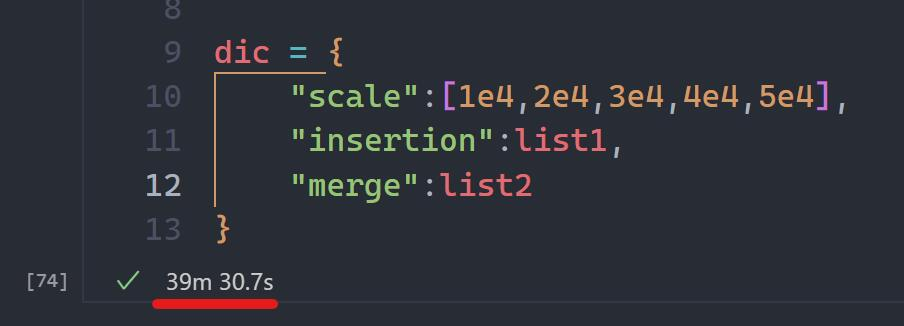
\includegraphics{./lab_1_files/1.jpg}

    \hypertarget{ux8c03ux8bd5ux8fc7ux7a0bux4e2dux9047ux5230ux7684ux95eeux9898}{%
\subsection{调试过程中遇到的问题}\label{ux8c03ux8bd5ux8fc7ux7a0bux4e2dux9047ux5230ux7684ux95eeux9898}}

\begin{enumerate}
\def\labelenumi{\arabic{enumi}.}
\tightlist
\item
  归并忘了咋写,看了看CLRS,又想起来了,还学会了哨兵写法。
\item
  python运行太慢,没办法解决,只能挂着运行。
\item
  pandas好久不用忘了咋写,看了看教程,复习了一下画图
\item
  插入排序规模5万时理论值与实际值相差甚大,不懂原因。想了好久,查阅各种资料,询问chatGPT,勉强拼凑出个人的浅薄见解
\end{enumerate}

\hypertarget{ux603bux7ed3ux5206ux6790}{%
\subsection{总结分析}\label{ux603bux7ed3ux5206ux6790}}

插入排序与归并排序的性能果真天差地别。无论是从时间复杂度公式来看,还是运行实践结果来看,归并排序的速度远高与插入排序,而且也同时具备稳定的效果。

但是归并排序是利用递归处理,递归调用需要一定的栈空间来保存函数调用的上下文信息,如果递归的深度过大,栈空间可能会不足导致栈溢出。此外,递归调用还需要在每次函数调用时保存一些状态信息,也会占用额外的空间。

本次实验,我进一步学会了用jupyter
notebook来进行科学运算探究。发现python写起来确实简单易懂,但是通过实验探究,发现python的运行效率确实低下(相较于Java,C系)。(但是运行时间长从另外一个角度看,可能并不是一件坏事,在它漫长的运行时间中,可以摸鱼喝茶等待,减少内卷,解放程序员\ldots)


    % Add a bibliography block to the postdoc
    
    
    
\end{document}
